\section{Gestión de Unidades de Aprendizaje}
    \subsection{Consulta de Unidades de Aprendizaje}
Para consultar Unidades de Aprendizaje el Jefe de División de Innovación Académica consulta un Plan de Estudios en la pantalla \hyperlink{consultarS}{\textit{Consultar Planes de Estudios}}:\\
\begin{figure}[H]
    \centering
    \hypertarget{consultarS}{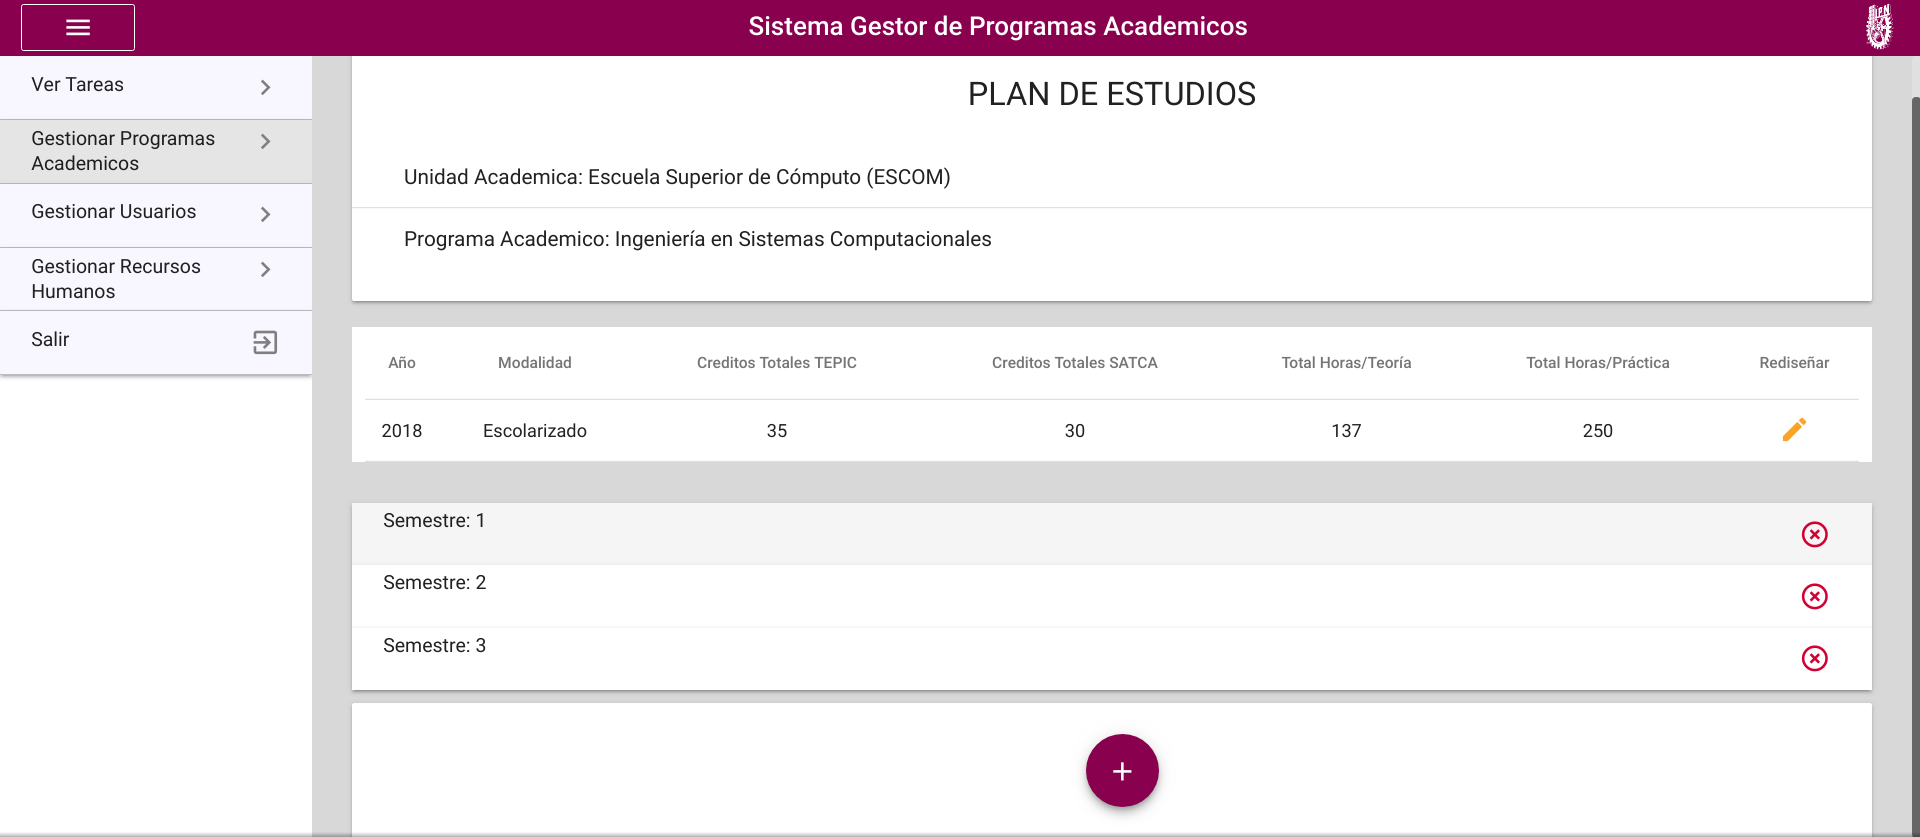
\includegraphics[width=0.7\linewidth]{images/GUA/consultarS}}
    \caption{Pantalla Consultar Plan de Estudios}
    \label{consultarS}
\end{figure}
\clearpage
Una vez en esta pantalla el usuario selecciona un semestre y este se expande desplegando las Unidades de Aprendizaje que tiene asociadas en la siguiente pantalla \hyperlink{consultarUA}{\textit{Consultar Planes de Estudios}}:\\
\begin{figure}[H]
    \centering
    \hypertarget{consultarUA}{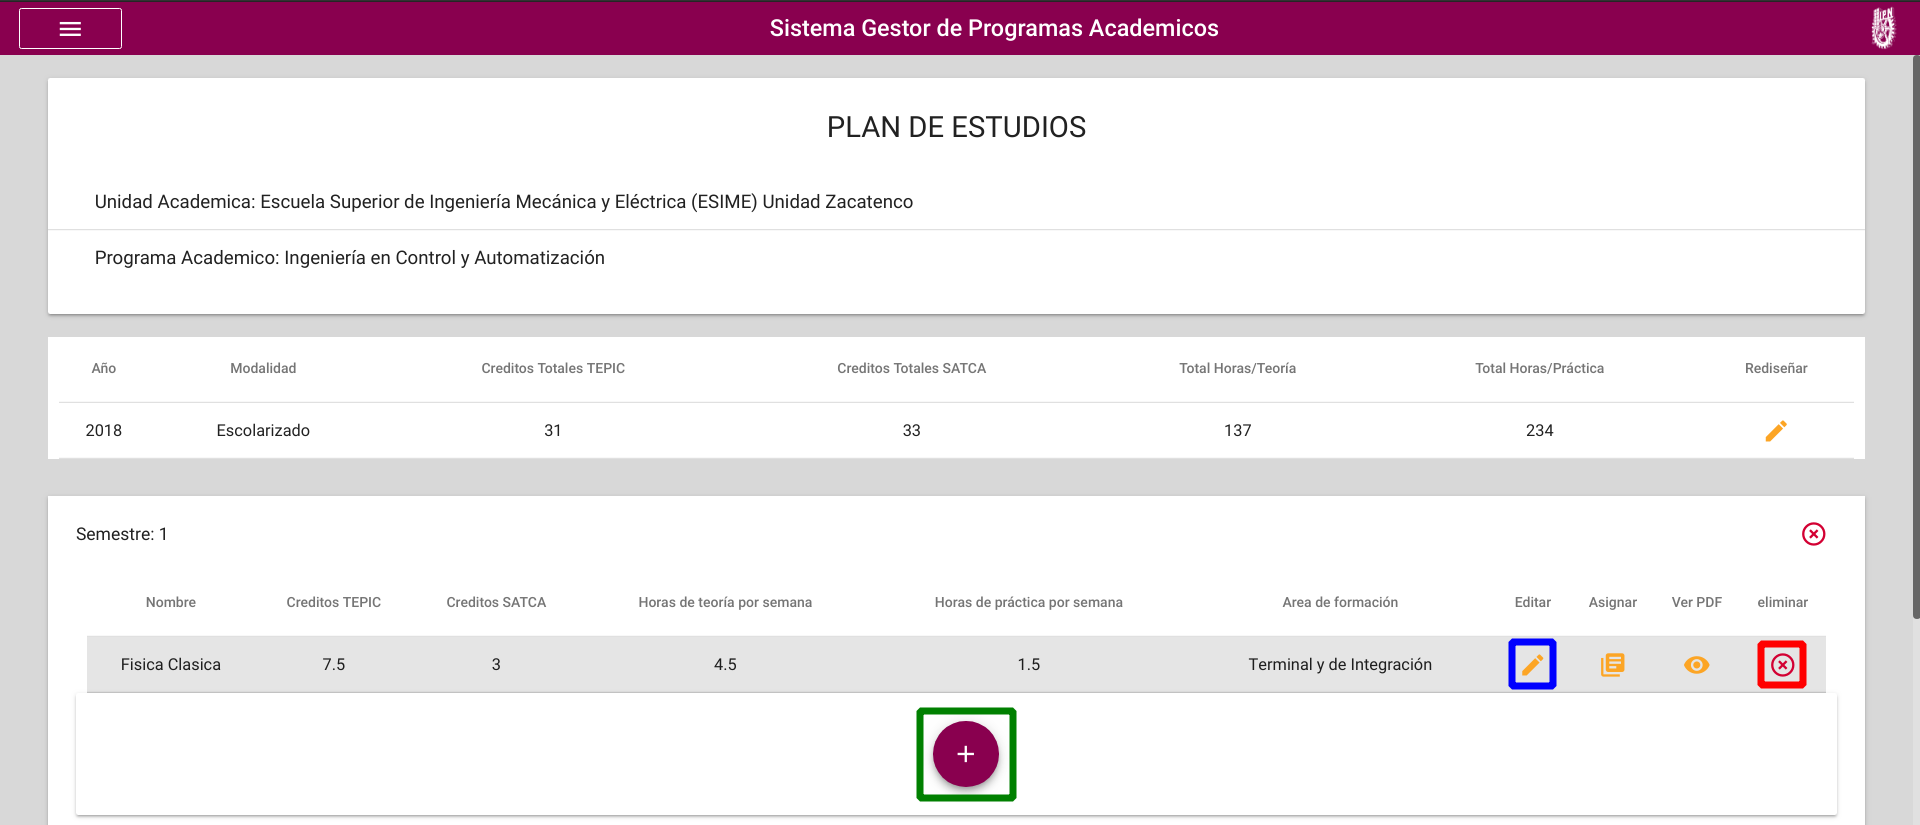
\includegraphics[width=0.7\linewidth]{images/GUA/consultarUA}}
    \caption{Pantalla Consultar Plan de Estudios Semestre expandido}
    \label{consultarUA}
\end{figure}
En esta ultima pantalla podemos realizar las tareas relacionadas a la gestión de Unidades de Aprendizaje, tendrá a su dispocisión las siguientes funciones relacionadas a los iconos en recuadros de colores para Registrar Unidad de Aprendizaje (verde), Editar Unidad de Aprendizaje (azul) y Eliminar Unidad de Aprendizaje (rojo).
\clearpage
\subsection{Registrar Unidades de Aprendizaje}
Cuando el Jefe de División de Innovación Académica presiona el icono de \IUbutton{+} en el recuadro verde en la pantalla \hyperlink{consultarUA}{\textit{Consultar Planes de Estudios}} lo lleva a la siguiente pantalla \hyperlink{registrarUA}{\textit{Registrar Unidad de Aprendizaje}}:\\
\begin{figure}[H]
    \centering
    \hypertarget{registrarUA}{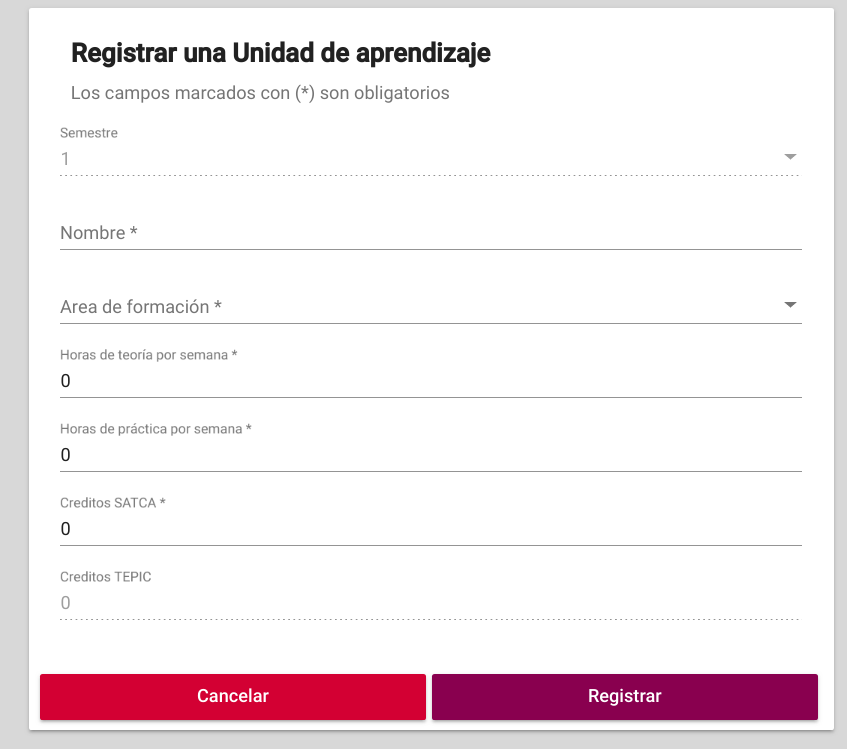
\includegraphics[width=0.7\linewidth]{images/GUA/registrarUA}}
    \caption{Pantalla Registrar Unidad de Aprendizaje}
    \label{registrarUA}
\end{figure}
\newpage
En donde tendrá que ingresar los campos de la nueva Unidad de Aprendizaje en el formulario para ser registrada.\\
Cuando ingrese un dato que no cumpla con el formato establecido el sistema se lo indicara con el siguiente mensaje:\\
\begin{figure}[H]
    \centering
    \hypertarget{invalidoR}{
\includegraphics[width=0.7\linewidth]{images/GUA/invalido}}
    \caption{Campo inválido: aparece cuando el formato o el tipo de dato es incorrecto}
    \label{invalidoR}
\end{figure}
Si usted se salta un campo o intenta finalizar si haber llenado los campos marcados con (*) que son obligatorios el sistema le mostrar el siguiente mensaje:\\
\begin{figure}[H]
    \centering
    \hypertarget{requeridoR}{
\includegraphics[width=0.7\linewidth]{images/GUA/requerido}}
    \caption{Campo requerido: aparece cuando un campo obligatorio se dejo vacío}
    \label{requeridoR}
\end{figure}
Cuando deseé finalizar el registro presione el botón \IUbutton{Registrar} en la parte inferior de la pantalla.\\
\begin{figure}[H]
    \centering
    \hypertarget{registrarBtnR}{
\includegraphics[width=0.7\linewidth]{images/GUA/registrarBtn}}
    \caption{Botones para finalizar o cancelar el registro}
    \label{registrarBtnR}
\end{figure}
Si la operación se pudo realizar aprecera el siguiente mensaje:\\
\begin{figure}[H]
    \centering
    \hypertarget{exito}{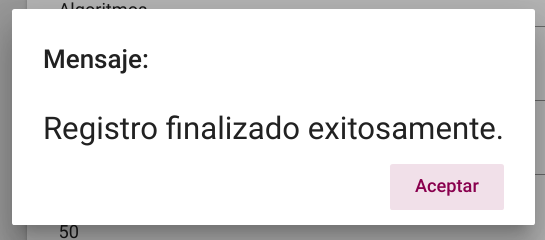
\includegraphics[width=0.7\linewidth]{images/GUA/exito}}
    \caption{Regisro Exitoso: aparece cuando su registro finaliza sin errores}
    \label{exito}
\end{figure}
En el caso de que ocurra un error aparecera este otro:\\
\begin{figure}[H]
    \centering
    \hypertarget{errorR}{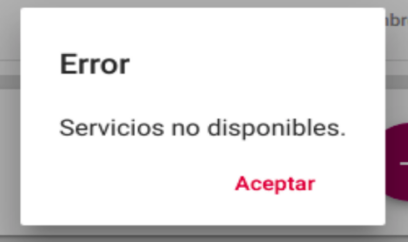
\includegraphics[width=0.7\linewidth]{images/GUA/error}}
    \caption{Error: Servicios no disponibles, aparece cuando ocurre un error en la conexión}
    \label{errorR}
\end{figure}
Si decide cancelar la operación necesitara presionar el botón \IUbutton{Cancelar} y aparecera el siguiente mensaje para pedir su confirmación:\\
\begin{figure}[H]
    \centering
    \hypertarget{cancelarR}{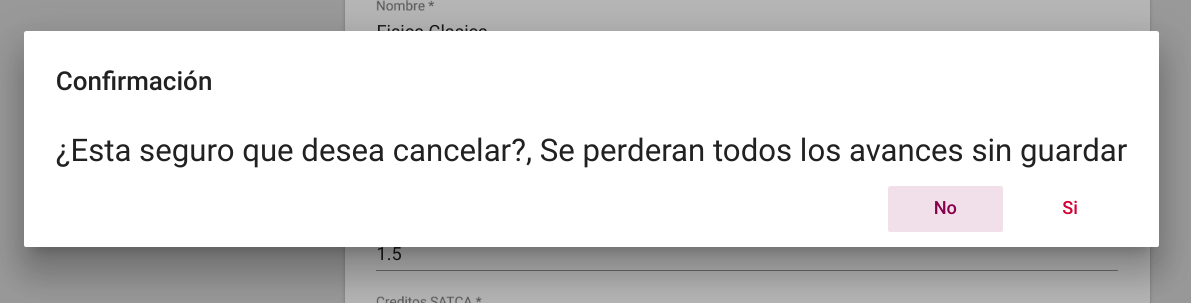
\includegraphics[width=0.7\linewidth]{images/GUA/cancelar}}
    \caption{Cancelación: este mensaje nos permite finalizar la operacion sin guardar}
    \label{cancelarR}
\end{figure}
\newpage
\subsection{Editar Unidades de Aprendizaje}
Cuando el Jefe de División de Innovación Académica presiona el icono de \BtnLapiz en el recuadro azul en la pantalla \hyperlink{consultarUA}{\textit{Consultar Planes de Estudios}} lo lleva a la siguiente pantalla a \hyperlink{editarUA}{\textit{Editar Unidad de Aprendizaje}}:\\
\begin{figure}[H]
    \centering
    \hypertarget{editarUA}{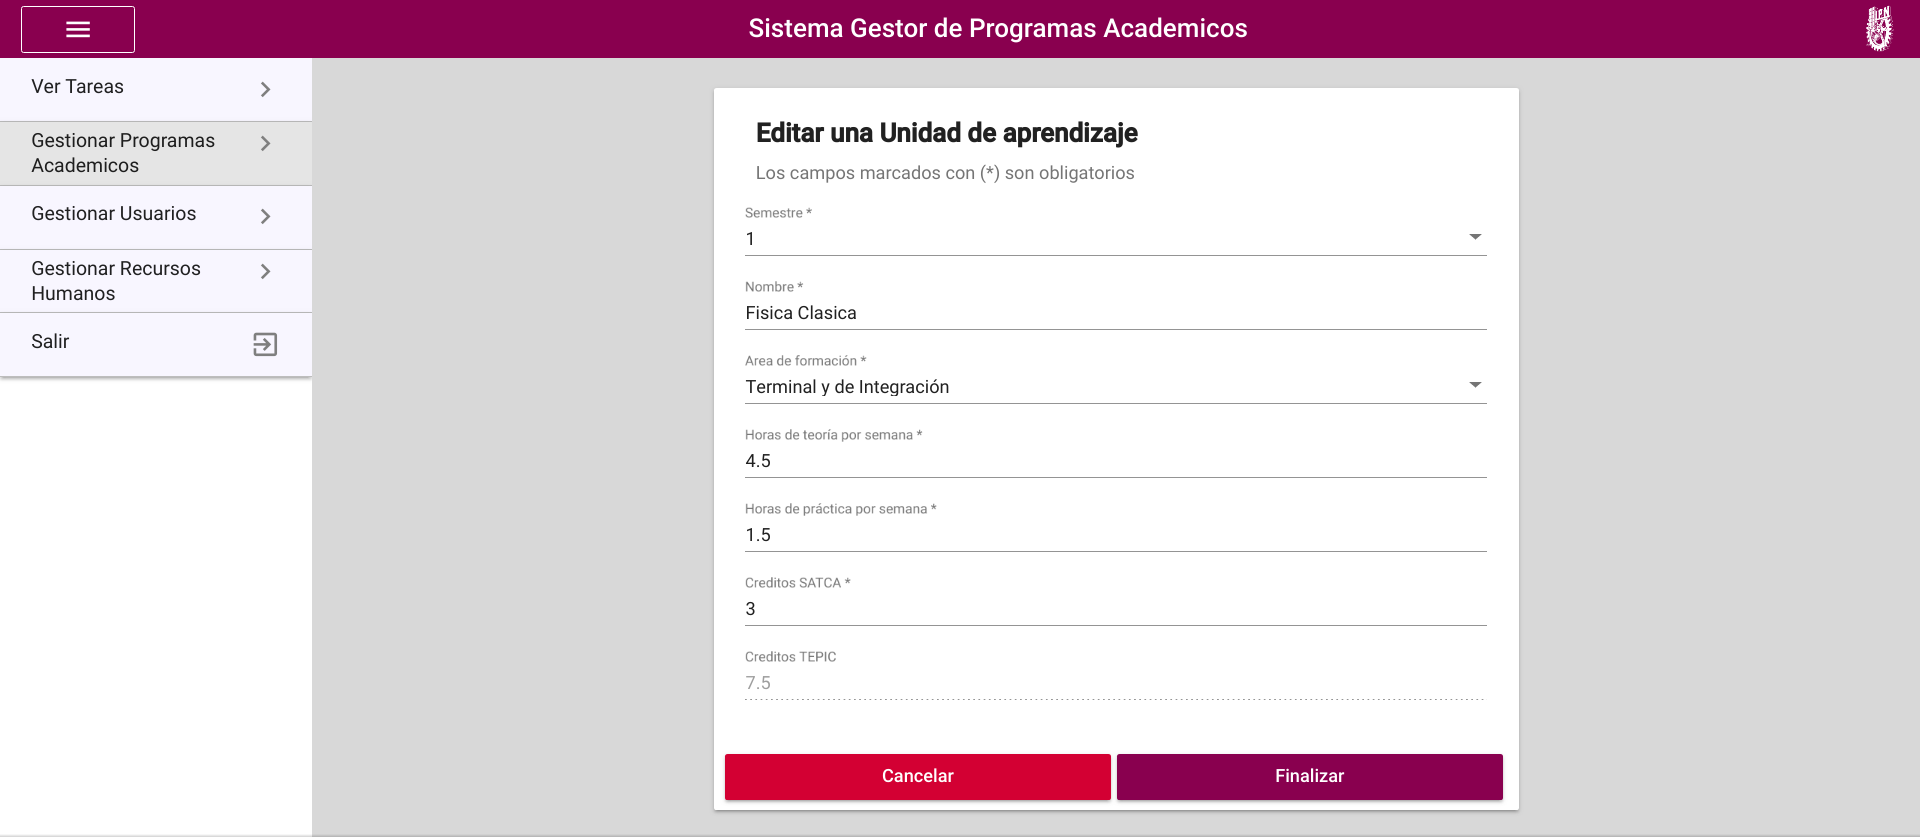
\includegraphics[width=0.7\linewidth]{images/GUA/editarUA}}
    \caption{Pantalla Editar Unidad de Aprendizaje}
    \label{editarUA}
\end{figure}
En donde se cargaran los datos de la Unidad de Aprendizaje seleccionada en la pantalla de \hyperlink{consultarUA}{\textit{Consultar Planes de Estudios}}  y llenará el formulario.\\
Durante la edición el sistema puede lanzar los siguientes mensajes:\\
Cuando modifique un dato y el nuevo valor no cumpla con el formato establecido para ese campo el siguiente mensaje sera mostrado:\\
\begin{figure}[H]
    \centering
    \hypertarget{invalidoE}{
\includegraphics[width=0.7\linewidth]{images/GUA/invalido}}
    \caption{Campo inválido: aparece cuando el formato o el tipo de dato es incorrecto}
    \label{invalidoE}
\end{figure}
Si un campo  marcado con (*), es decir obligatorio, es dejado en blanco, el sistema le mostrar el siguiente mensaje:\\
\begin{figure}[H]
    \centering
    \hypertarget{requeridoE}{
\includegraphics[width=0.7\linewidth]{images/GUA/requerido}}
    \caption{Campo requerido: aparece cuando un campo obligatorio se dejo vacío}
    \label{requeridoE}
\end{figure}
Cuando haya terminado de realizar las modificaciones pertinentes presione el botón \IUbutton{Finalizar} en la parte inferior de la pantalla.\\
\begin{figure}[H]
    \centering
    \hypertarget{finalizarBtnE}{
\includegraphics[width=0.7\linewidth]{images/GUA/finalizarBtn}}
    \caption{Botones para finalizar las operaciones de Edición}
    \label{finalizarBtnE}
\end{figure}
Si la operación se pudo concluir sin erroes el siguiente mensaje sera desplegado:\\
\begin{figure}[H]
    \centering
    \hypertarget{modificacion}{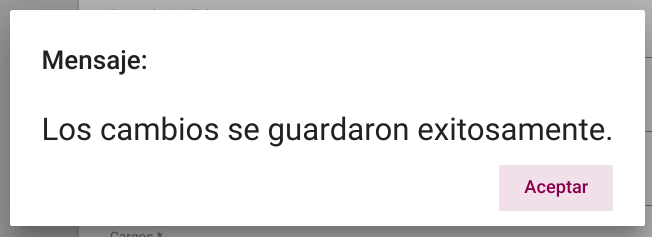
\includegraphics[width=0.7\linewidth]{images/GUA/modificacion}}
    \caption{Modificación exitosa: mensaje para notificar del exito de la operación}
    \label{modificacion}
\end{figure}
En el caso de que ocurra un error aparecera este otro:\\
\begin{figure}[H]
    \centering
    \hypertarget{errorE}{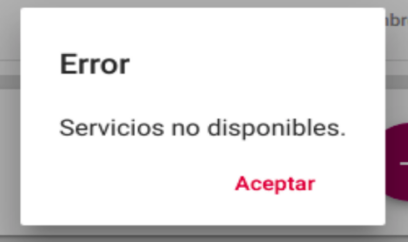
\includegraphics[width=0.7\linewidth]{images/GUA/error}}
    \caption{Error: Servicios no disponibles, aparece cuando ocurre un error en la conexión}
    \label{errorE}
\end{figure}
Si decide cancelar la operación necesitara presionar el botón \IUbutton{Cancelar} y aparecera el siguiente mensaje para pedir su confirmación:\\
\begin{figure}[H]
    \centering
    \hypertarget{cancelarE}{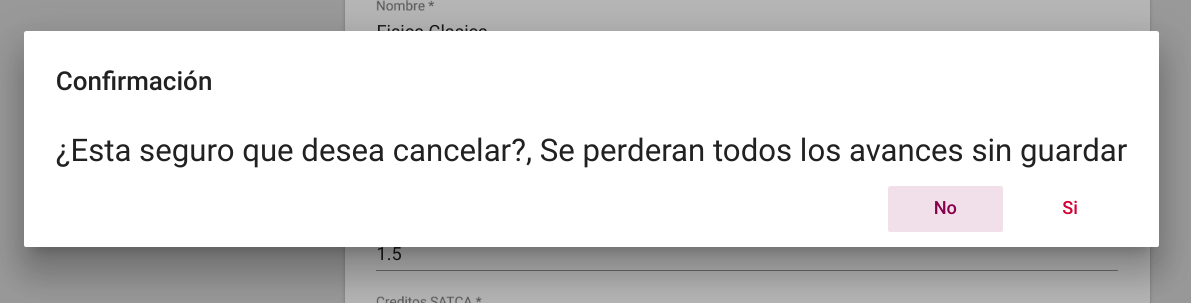
\includegraphics[width=0.7\linewidth]{images/GUA/cancelar}}
    \caption{Cancelación: este mensaje nos permite finalizar la operacion sin guardar}
    \label{cancelarE}
\end{figure}
\newpage
\subsection{Eliminar Unidades de Aprendizaje}
Cuando el Jefe de División de Innovación Académica quiera eliminar una Unidad de Aprendizaje presiona el botón \IUbutton{X} en el recuadro rojo en la pantalla \hyperlink{consultarUA}{\textit{Consultar Planes de Estudios}} y se le mostrara el siguietne mensaje solicitando confirmación:\\
\begin{figure}[H]
    \centering
    \hypertarget{EliminarUA}{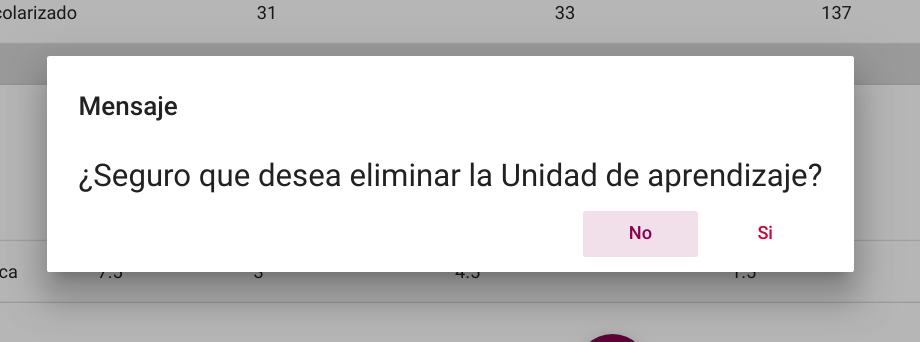
\includegraphics[width=0.7\linewidth]{images/GUA/EliminarUA}}
    \caption{Eliminar Unidad de Aprendizaje: solicita confirmación para eliminar permanentemente una Unidad de Aprendizaje}
    \label{EliminarUA}
\end{figure}